\section{A Joint Evaluation of Executed Cover}\label{sec:experiment}
\textbf{The dispatcher changes residual inference and resource use; business correctness needs its own endpoint.}
Table~\ref{tab:study-map} lists the populations used here. Each keeps its own denominators, and only the families named there are primary.

\begin{table}[t]\centering\footnotesize
\caption{Study map. Each population answers one question and keeps its own denominators and statistical role.}\label{tab:study-map}
\setlength{\tabcolsep}{3pt}
\begin{tabularx}{\columnwidth}{@{}P{.2\columnwidth}P{.25\columnwidth}Y@{}}\toprule
Study & Population; observer & Question; role \\\midrule
Live timing (\S\ref{sec:cover-study}) & 3,000 episodes + 600 shadow chains; call windows, TLS record times & Does the dispatcher expose cover? Primary families P, R, C \\\addlinespace[2pt]
Record-only (\S\ref{sec:no-call}) & Same episodes; no call boundaries & How much survives without supplied boundaries? Retrospective; one primary pair \\\addlinespace[2pt]
State control (\S\ref{sec:business}; S1) & 3,600 episodes; call windows, sizes only & Does goal completion miss collateral state? Primary state family \\\addlinespace[2pt]
Forwarding pilot (S10) & 3,120 local + 192 hosted & Feedback attribution; inconclusive, supplement only \\\bottomrule
\end{tabularx}\end{table}


\paragraph{Statistical conventions}
These apply throughout this section and are not repeated. \emph{Sel.}\ is the attack chosen on validation data before test scoring; primary tests use only these choices. \emph{Max} is the largest test count in a finite attack suite; it is descriptive and is not an upper bound on inference. \emph{Exploratory} marks an analysis designed after test results were seen. Intervals condition on the fitted attacks and the designed workload. All runs are on one host over loopback with synthetic tools and fixtures reused across studies; Section~\ref{sec:validity} lists what this does not test.

\begin{figure}[t]\centering
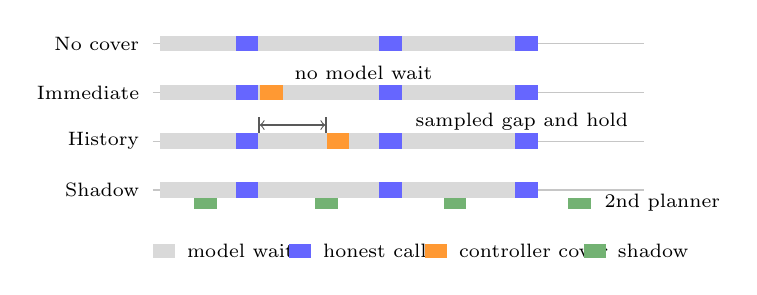
\begin{tikzpicture}[x=.48cm,y=.62cm,font=\scriptsize]
\def\bar#1#2#3#4{\fill[#4] (#1,#3-.16) rectangle (#2,#3+.16);}
\foreach \y/\n in {4/No cover,3/Immediate,2/History,1/Shadow}{
 \node[anchor=east] at (-.1,\y) {\n};
 \draw[gray!45] (0,\y)--(13,\y);
 \bar{0.2}{2.2}{\y}{gray!30}\bar{2.2}{2.8}{\y}{blue!60}
 \bar{2.8}{6.0}{\y}{gray!30}\bar{6.0}{6.6}{\y}{blue!60}
 \bar{6.6}{9.6}{\y}{gray!30}\bar{9.6}{10.2}{\y}{blue!60}}
% immediate cover: right after the honest response
\bar{2.85}{3.45}{3}{orange!80}
\node[anchor=west] at (3.5,3.4) {no model wait};
% history cover: after a sampled gap
\bar{4.6}{5.2}{2}{orange!80}
\draw[|<->|,gray!70!black] (2.8,2.33)--(4.6,2.33);
\node[anchor=west] at (6.7,2.4) {sampled gap and hold};
% shadow chain: its own model waits
\foreach \a in {1.1,4.3,7.7,11.0}{\fill[green!45!black!55] (\a,.62) rectangle (\a+.6,.84);}
\node[anchor=west] at (11.7,.73) {2nd planner};
% legend
\begin{scope}[yshift=-.25cm]
\fill[gray!30] (0,0) rectangle (.6,.3); \node[anchor=west] at (.65,.15) {model wait};
\fill[blue!60] (3.6,0) rectangle (4.2,.3); \node[anchor=west] at (4.25,.15) {honest call};
\fill[orange!80] (7.2,0) rectangle (7.8,.3); \node[anchor=west] at (7.85,.15) {controller cover};
\fill[green!45!black!55] (11.4,0) rectangle (12.0,.3); \node[anchor=west] at (12.05,.15) {shadow};
\end{scope}
\end{tikzpicture}
\caption{Dispatchers in the live study. Honest calls follow a model wait. Immediate cover follows the previous response without one, which label-free gap removal exploits. History-matched cover samples a training gap and response hold. Shadow calls come from a second planner, so their gaps are model waits too.}\label{fig:dispatch}
\end{figure}

\subsection{Actual dispatch and timing-aware attacks}\label{sec:cover-study}
\textbf{Cover inherits the timing of whatever process dispatches it.}
Two fixed-weight planners, Qwen3:8B and Llama3.1:8B, each execute 300 fixtures in five conditions, yielding 3,000 main episodes and 600 additional shadow chains. The six business actions use seven MCP services through LangGraph over TLS~1.3/HTTP/2; the services stand for third-party tools that offer no cover terminator (Table~\ref{tab:cover-necessity}). Partitions contain 120 training, 60 validation and 120 paired test fixtures per cell. The task label is requested intent; failures remain included. Cover executes on an isolated clone and its responses are hidden from the real planner.

The four cover arms vary only the dispatcher (Figure~\ref{fig:dispatch}). \emph{Immediate} cover follows an honest response directly. \emph{History} cover samples a training-only honest gap and service duration, waits in real time and holds the response for the sampled minimum; the \emph{sequential} variant blocks the real chain, the \emph{concurrent} one overlaps real model inference. \emph{Shadow} runs a complete second planner on an independent, uniformly drawn ticket; a fair draw decides which chain starts first. Calls to the same service serialize. The observer receives destinations, ciphertext bytes, TLS record completion times and supplied episode/call windows; Section~\ref{sec:no-call} withdraws the call windows.

\begin{table*}[t]\centering\small
\caption{Joint evaluation of the five live policies; 120 test fixtures per row, single host over loopback, synthetic tools. Sel.\ S/A: validation-selected size-only / adaptive attack (primary). Max: largest test count in the frozen suite (descriptive). GMM: label-free removal. Ref.: uniform six-class reference 20/120, or for shadow the realized pair-ambiguity floor (Table~\ref{tab:shadow-floor}). Bytes: whole-connection / call-window factors. Tokens include both planners. Goal and State are separate counts from this cohort; the state-control cohort (Supplement S1) has its own counts.}\label{tab:live-timing-main}
\setlength{\tabcolsep}{4pt}
\begin{tabularx}{\textwidth}{@{}lYrrrrrrr@{}}\toprule
Planner & Policy & Sel. S/A & Max & GMM & Ref. & Bytes$\times$ & Tokens$\times$ & Goal/State \\\midrule

Qwen3:8B & No cover & 117/117 & 117 & -- & 20 & 1.00/1.00 & 1.00 & 113/114 \\
Qwen3:8B & Immediate & 75/112 & 112 & 112 & 20 & 1.15/1.33 & 1.00 & 111/112 \\
Qwen3:8B & History, sequential & 76/93 & 99 & 53 & 20 & 1.15/1.32 & 1.00 & 112/113 \\
Qwen3:8B & History, concurrent & 66/99 & 99 & 38 & 20 & 1.15/1.33 & 1.00 & 111/112 \\
Qwen3:8B & Planner shadow & 54/54 & 70 & 34 & 70.5 & 1.31/1.68 & 2.01 & 112/113 \\
Llama3.1:8B & No cover & 110/110 & 112 & -- & 20 & 1.00/1.00 & 1.00 & 82/70 \\
Llama3.1:8B & Immediate & 80/108 & 108 & 108 & 20 & 1.13/1.27 & 1.01 & 83/67 \\
Llama3.1:8B & History, sequential & 82/104 & 104 & 14 & 20 & 1.13/1.26 & 1.01 & 84/67 \\
Llama3.1:8B & History, concurrent & 68/106 & 106 & 66 & 20 & 1.13/1.27 & 1.02 & 82/67 \\
Llama3.1:8B & Planner shadow & 64/64 & 64 & 43 & 70.5 & 1.35/1.71 & 1.99 & 82/67 \\
\bottomrule\end{tabularx}\end{table*}


\paragraph{Immediate cover: a calibration baseline}
A label-free two-component mixture over training gaps selects the short-gap component for removal; a classifier trained on no-cover traffic decodes the rest. This restores 112/120 and 108/120 correct predictions, against selected non-timing attacks at 75 and 80, and meets the prespecified replication rule in both models after Holm correction. The result confirms the mechanism rather than reporting a new weakness: a controller that skips the model wait is removable. Independent TCP reassembly matches all 773,450 recorded TLS record types, lengths and counts, and refitting the mixture on packet-capture clocks reproduces both scores (Supplement S2).

\paragraph{History matching removes the shortcut, not the signal}
History sampling defeats the simple mixture, but adapted context removal or joint decoding still recognizes 93/120 and 104/120 sequential executions, against selected non-timing attacks at 76 and 82 (Holm $p=.0559$ and $.00078$). Concurrent dispatch gives 99/120 and 106/120 against 66 and 68; both 27.5- and 31.7-point advantages pass correction. The policy controls minimum waits, not achieved timing: Qwen's mean sampled hold of 40.5\,ms becomes 100.4\,ms sequential and 171.2\,ms concurrent at the record observer. A failed simple attack is therefore not evidence of concealment. Llama's sequential mixture deletes 477/634 honest calls while detecting only 64/182 cover calls, which explains its 14/120, while adapted joint decoding on the same traces reaches 104/120.

\begin{table}[t]\centering\footnotesize
\caption{Pair-ambiguity floor $P^*(k)$ for $k$ shadow planners and six classes, computed exactly (\texttt{experiment/shadow\_floor.py}). \emph{iid}: shadow labels drawn uniformly; \emph{distinct}: drawn without replacement from classes other than the real one. Tokens are nominal planner multiples. Only $k=1$, iid, was run.}\label{tab:shadow-floor}
\setlength{\tabcolsep}{4pt}
\begin{tabular}{@{}rrrrl@{}}\toprule
$k$ & iid & distinct & Tokens$\times$ & Live result ($k=1$) \\\midrule
0 & 1.000 & -- & 1 & \\
1 & .583 & .500 & 2 & Max 70 / 64 of 120 \\
2 & .491 & .333 & 3 & \\
3 & .456 & .250 & 4 & \\
4 & .428 & .200 & 5 & \\\midrule
\multicolumn{5}{@{}l}{Realized $k=1$ floor on the test split: 70.5/120 (21 matching labels)} \\\bottomrule
\end{tabular}\end{table}


\paragraph{Planner shadow sits at its pair-ambiguity floor}
Suppose an attacker separates the real chain from $k$ shadow chains perfectly and recovers every chain's label, but cannot tell which chain is real. If the real chain is exchangeable with the shadows, the best guess is the modal label, which succeeds with probability $P^*(k)=\mathbb{E}[\max_c n_c]/(k+1)$ for $n_c$ chains labeled $c$. With one shadow and six uniform classes, $P^*(1)=1/6+\tfrac{5}{6}\cdot\tfrac12=7/12$ (Table~\ref{tab:shadow-floor}). On the realized test split, 21 of 120 shadow labels match the real one, so the floor is 70.5/120.

The strongest tested attack, a size/destination random forest, scores 70/120 for Qwen and 64/120 for Llama; the validation-selected attacks score 54 and 64. Neither exceeds the floor, so the tested attacks are no more accurate than an attacker who already knew both tasks, and the 16.7\% uniform reference is the wrong comparison for this design. The floor is not a bound: real tickets are reused fixtures with their own cache histories, so exchangeability is an idealization, and an attacker who learns role cues could exceed it. A chain-separation attack scores 49 and 34 and recovers the real chain exactly in only 29 and 32 fixtures. Which chain the attacker can identify is a separate question. Among the 99 fixtures whose labels differ, the aggregate counts bound the real-label accuracy of the forest only to $[49,70]/99$ and $[43,64]/99$. An exact role test against 50\% needs the saved per-fixture predictions and is part of the artifact (Section~\ref{sec:validity}). The prespecified equivalence family E is degenerate here, because both selectors chose the same attack and every pair ties; we do not count it as evidence.

Shadow costs 2.01/1.99 times the model tokens, 1.68/1.71 times the call-window bytes, and raises mean real-chain time from 2.91/3.33\,s to 4.80/3.94\,s. Table~\ref{tab:shadow-floor} shows the trade-off this implies: each further independent shadow adds one planner's work and lowers the floor slowly, whereas drawing shadow labels without replacement from the other classes lowers it to $1/(k+1)$ at no extra cost. Neither variant was run; both are the next measurements this design calls for. Supplement S2 retains every attack, test and cost.

\subsection{Recognition without supplied call boundaries}\label{sec:no-call}
\textbf{Without call boundaries, the prespecified removal attack loses its advantage.}
We reanalyze all 3,000 episodes from complete encrypted connections, including initialization and closing records. The attacker receives relative record times, directions, ciphertext lengths and destinations, but no call starts or ends, operation names, role labels or HTTP stream assignment. Whole-episode association remains supplied, so this withdraws call boundaries, not task localization. A per-connection idle-gap rule proposes events, with five gaps from 5 to 250\,ms competing on validation accuracy; raw-record classifiers skip eventization. LR and RF use destination summaries and early/late event sequences, with and without timing, and a training-only mixture removes short-gap events before a no-cover classifier. This is a retrospective, fixed-protocol analysis of reused fixtures; the immediate-arm pair is its only primary test, with Holm over the two models.

\begin{table}[t]\centering\small
\caption{No supplied call boundaries; whole-episode association remains supplied. B/R: validation-selected idle-grid baseline and removal attacks (primary pair: immediate). Max: largest test count over both suites, including the exploratory protocol-aware eventizer designed after the idle-grid results were seen (descriptive). Counts out of 120; uniform reference 20.}\label{tab:no-call-main}
\setlength{\tabcolsep}{4pt}
\begin{tabularx}{\columnwidth}{@{}Yrrrr@{}}\toprule
 & \multicolumn{2}{c}{Qwen} & \multicolumn{2}{c}{Llama} \\\cmidrule(lr){2-3}\cmidrule(l){4-5}
Policy & B/R & Max & B/R & Max \\\midrule
No cover & 115/109 & 117 & 108/101 & 112 \\
Immediate & 80/69 & 91 & 90/86 & 97 \\
History, sequential & 73/74 & 75 & 88/56 & 93 \\
History, concurrent & 56/61 & 62 & 78/62 & 88 \\
Planner shadow & 69/65 & 73 & 69/56 & 69 \\
\bottomrule\end{tabularx}\end{table}

On immediate cover, selected removal recognizes 69/120 and 86/120 tasks, against baselines of 80 and 90: paired differences of $-9.2$ and $-3.3$ points (Holm $p=.025$ and $.54$). Removal is worse than the baseline for Qwen and indistinguishable for Llama, so the call-window removal advantage does not carry over to this pipeline. An exploratory eventizer, designed after these results were seen, uses the public request-padding quantum and MCP setup sequence to mark proposed requests and responses; it reads no call truth. It raises Qwen's removal count from 68 to 91 but lowers Llama's from 90 to 87. Because the representations differ, the gap from the call-window counts is not a pure causal effect of boundaries. Its event recovery is poor: protocol-event F1 is 0.295 and 0.380 at IoU .5 on immediate cover, so task recognition here does not imply recovering calls. For shadow, the Qwen maximum of 73/120 over 52 candidates is 2.5 fixtures above the realized floor; the selected attacks (69 and 69) are below it. Supplement S3 gives the protocol and the event audit.

\subsection{Business constraints and the protection decision}\label{sec:business}
Every live cover arm executes in isolated state and hides cover feedback from the real planner. Table~\ref{tab:live-timing-main} reports goal/state counts on the same fixtures as inference and costs. Shadow outcomes are 112/113 for Qwen and 82/67 for Llama, versus no-cover 113/114 and 82/70. These are different endpoint counts: a correctly preserved state need not contain a successful intended action. Low Llama baseline performance and changed planning paths limit business-equivalence conclusions.

The earlier six-policy study supplies a deliberately adverse state control (Supplement S1). Read/proxy/hidden-isolated cover retains Qwen state correctness at 115--116/120. Live writes can alter other objects and reduce it to 7/120; 95 of 102 completed Qwen tasks have collateral errors. Llama's corresponding counts are 3/120 intact and 73 of 76 completed tasks with collateral errors. The harm direction is built into that stress condition: it tests whether the evaluation records forbidden effects, not how often production writes cause them.

The combined decision is concrete. Immediate cover leaves high inference after removal. Historical dispatch changes that attack but retains substantial adapted inference. Shadow execution trades model work for a trace whose strongest tested attack sits at the design's pair-ambiguity floor; lowering that floor needs more shadows. An adverse write can fail the state contract even when the requested goal passes. Choosing a policy requires stating acceptable inference, task, state and resource tolerances rather than comparing a single accuracy decrease.
